\documentclass[a4paper, 12pt]{article}
\author{Justin L. Clough, 
        Irina K. Tezaur,
        Assad A. Oberai}
\title{Convergence Study for Tetrahedrons with Composite, Quadratic, and Linear Shape Functions in Bending}
\usepackage[margin=1in]{geometry}
\usepackage{float}
\usepackage{subfigure}
\usepackage[justification=centering]{caption}
\usepackage{enumerate}
\usepackage{multirow}
\usepackage{listings}
\lstset{
    escapechar=`,
    language=C++,
    numbers=left,
    tabsize=2,
    prebreak=\raisebox{0ex}[0ex][0ex]{\ensuremath{\hookleftarrow}},
    frame=single,
    breaklines=true,
}
\usepackage{graphicx}
\graphicspath{ {./images/} }
\usepackage{nameref}
\usepackage{amsmath}
\usepackage{amssymb}
\usepackage{amsfonts}
\usepackage[linesnumbered,ruled]{algorithm2e}
\usepackage{tikz}
\usetikzlibrary{calc,patterns,decorations.pathmorphing,decorations.markings,positioning,automata}
\usepackage{pgfplots}
\pgfplotsset{compat=1.5}
\usepackage{pgfplotstable}
\usepackage{makecell}
\usepackage{verbatim}
\usepackage[super]{nth}

\begin{document}
\maketitle

\begin{abstract}
The convergence of tetrahedral elements with
\nth{2} order shape functions are compared to those with composite
and linear shape functions
in a beam bending problem.
A linear elastic material model was used
and no time components were considered.
The geometry was a beam with a square cross-section and 
aspect ratio of 100.
The beam was cantilevered on one end and received a 
shearing traction at the other. 
The tip deflection of the finite element solutions were
compared to that from Euler-Bernoulli beam theory. 
Tetrahedrons with \nth{2} order and composite shape functions under-predicted
the theoretical tip displacement by less than 1\% with 2 elements  
through the thickness of the beam;
elements with linear shape functions under-predicted 
the theoretical tip displacement by 84\% with 8 elements through the thickness.
Tetrahedrons with \nth{2} order shape functions under-predicted 
the peak bending stress by 4\% in tension and 7\% in compression
with 8 elements through the thickness.
Tetrahedrons with composite shape functions under-predicted 
the peak bending stress by 10\% in tension and 0.4\% in compression
with 8 elements through the thickness.
Performance of iterative solvers for both the 
quadratic and composite element types are discussed.

\end{abstract}

\section{Introduction}
The performance of tetrahedron elements with \nth{2} order shape functions
was compared to that of elements with composite
(discussed in \cite{bib:composite_tet})
and linear shape functions in a beam-bending problem.
The mesh was refined such that the aspect ratio of the elements
stayed at 10 as the number of elements through the thickness was increased.
The theoretical deflection from Euler-Bernoulli beam theory was used to
compared the finite element results.

\section{Methods}
The problem geometry was a beam with a square cross-section.
The cross-section was 0.01 m $ \times $ 0.01 m; 
the beam was 1 m long in the $Y$ direction.
The other edges of the beam were aligned with the $X$ and $Z$ axes.

A linear elastic material model was used. 
Young's Modulus was 80,000 Pa;
Poisson's ratio was 0.25.
No time components were considered
and only the static solution was calculated.

The square face with normal in the negative $Y$ direction had 
all degrees of freedom fixed to act as a cantilever support. 
The face on the other end of the beam received a 
traction of 0.01 $\frac{N}{m^2}$ in the $Z$ direction.
From Euler-Bernoulli beam theory, the tip deflection
is modeled as:

\begin{equation}
  \delta = \frac{F L^3}{3 E I}
  \label{eq:EB_deflection}
\end{equation}

\noindent
where 
$F$ is the total force acting at the tip of the beam, 
$L$ is the length of the beam,
$E$ is Young's Modulus for the beam's material,
and
$I$ is the second moment of the cross-sectional area.
Evaluating Equation (\ref{eq:EB_deflection}) for the
given parameters of the problem, 
the theoretical tip deflection is 5.0 mm.
The peak bending stress, $\sigma_b$, was modeled as:

\begin{equation}
\sigma_b = \frac{M c}{I}
\end{equation}

\noindent
where $M$ is the bending moment, 
$c$ is the maximum distance from the bending axis to a point on the beam.
With the parameters of the problem, $\sigma_b = \pm 6$ 
with ``+'' taken as tension.


A mesh was constructed to approximate the beam geometry
and used only tetrahedral elements.
The convergence of 
tetrahedrons with \nth{2} order (quadratic tet10 elements),
composite, and linear shape functions
were separately measured.
An element aspect ratio of 10 was used for all meshes
and the number of elements through the thickness of the beam was increased.
Figure \ref{fig_mesh} shows an example mesh with 2 elements through the 
thickness. 
Additional images of the other meshes are shown in Appendix \ref{app_mesh_images}
All systems were solved with iterative solvers.

\begin{figure}[H]
  \centering
  \subfigure[Side View.]
  {
    
\includegraphics[width=1.0\textwidth]
    {beam_2}
  }
  \subfigure[End View.]
  {
    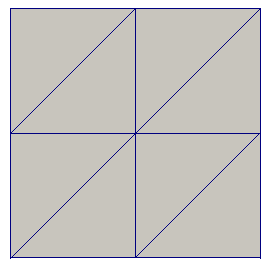
\includegraphics
    {beam_2_end}
  }
  \caption{Mesh for beam of size $0.01 \times 0.01\times 1$ with $2\times 2\times 20$ elements.}
  \label{fig_mesh}
\end{figure}

\section{Results}
The tip deflections from the finite element solutions
are shown with respect to the number of degrees of freedom 
in Figure \ref{fig:convergence};
a focused view of just the composite and quadratic 
elements is shown in Figure \ref{fig:quad_comp_foucs}.
Four meshes were constructed with 1, 2, 4, and 8 elements
through the thickness.

\begin{figure}[H]
  \centering
    \begin{tikzpicture}
      \begin{axis}[
        legend pos=outer north east,
        legend cell align={left},
        grid=both,
        grid style={line width=.1pt, draw=gray!10},
        major grid style={line width=.2pt,draw=gray!50},
        xtick={},
        ytick={},
        minor tick num=5,
        title=Convergence of Tip Deflection,
        xlabel=Degrees of Freedom,
        ylabel={Tip Deflection [mm]} ]
        \addplot table {quadratic_data_beam.txt};
          \addlegendentry{Quadratic}
        \addplot table {composite_data_beam.txt};
          \addlegendentry{Composite}
        \addplot table {linear_data_beam.txt};
          \addlegendentry{Linear}
      \end{axis}
    \end{tikzpicture}
  \caption{Tip deflection for beam geometry with composite, quadratic, and linear elements.
           The number of elements through the thickness was 1, 2, 4, and 8.
           Analytical solution is 5.0 mm.}
  \label{fig:convergence}
\end{figure}

\begin{figure}[H]
  \centering
    \begin{tikzpicture}
      \begin{axis}[
        legend pos=outer north east,
        legend cell align={left},
        grid=both,
        grid style={line width=.1pt, draw=gray!10},
        major grid style={line width=.2pt,draw=gray!50},
        xtick={},
        ytick={},
        minor tick num=5,
        title=Convergence of Tip Deflection,
        xlabel=Degrees of Freedom,
        yticklabel style={/pgf/number format/.cd,fixed,fixed zerofill,precision=2,/tikz/.cd},
        ylabel={Tip Deflection [m]} ]
        \addplot table {quadratic_data_beam.txt};
          \addlegendentry{Quadratic}
        \addplot table {composite_data_beam.txt};
          \addlegendentry{Composite}
      \end{axis}
    \end{tikzpicture}
  \caption{Tip deflection for beam geometry with composite and quadratic elements.
           The number of elements through the thickness was 1, 2, 4, and 8.
           Analytical solution is 0.1 m.}
  \label{fig:quad_comp_foucs}
\end{figure}

The quadratic and composite tet10 elements underestimated the tip deflection 
by 0.1\% of the analytical solution with 4 elements through 
the thickness. 
The linear elements underestimated 
the analytical solution by more than 83.5\% in all cases.
The peak compression and bending stresses for
the composite and quadratic elements are shown in 
Figure \ref{fig:stresses}.

\begin{figure}[H]
  \centering
    \begin{tikzpicture}
      \begin{axis}[
        legend pos=outer north east,
        legend cell align={left},
        grid=both,
        grid style={line width=.1pt, draw=gray!10},
        major grid style={line width=.2pt,draw=gray!50},
        xtick={},
        ytick={-6,-4,...,6},
        ymax=7,
        ymin=-7,
        minor tick num=5,
        title=Convergence of Bending Stress,
        xlabel=Degrees of Freedom,
        ylabel={Stress at Beam Root [Pa]} ]
        \addplot table {quad_tension_data.txt};
          \addlegendentry{Quadratic-Tension}
        \addplot table {composite_tension_data.txt};
          \addlegendentry{Composite-Tension}
        \addplot table {quad_compression_data.txt};
          \addlegendentry{Quadratic-Compression}
        \addplot table {composite_compression_data.txt};
          \addlegendentry{Composite-Compression}
      \end{axis}
    \end{tikzpicture}
  \caption{Bending stress for beam with composite and quadratic elements.
           The number of elements through the thickness was 1, 2, 4, and 8.
           Analytical solution is $\pm$ 6 Pa.}
  \label{fig:stresses}
\end{figure}

The quadratic elements underestimated
the peak bending stress by 4\% in tension and 7\% in compression 
with 8 elements through the thickness.
The composite elements underestimated
the peak bending stress by 10\% in tension and 0.4\% in compression
with 8 elements through the thickness.
A \texttt{Block GMRES} method was used to solve the linear systems;
a relative tolerance of $10^{-6}$ was used for all solutions.
More details of the solver and preconditioner are shown in 
the sample input file in Appendix \ref{app_input_file}.
The number of steps to solve each system is shown in 
Figure \ref{fig:iterations}.


\begin{figure}[H]
  \centering
    \begin{tikzpicture}
      \begin{loglogaxis}[
        legend pos=outer north east,
        legend cell align={left},
        grid=both,
        grid style={line width=.1pt, draw=gray!10},
        major grid style={line width=.2pt,draw=gray!50},
        xtick={},
        ytick={},
        minor tick num=5,
        title=Iterations to Solve Systems,
        xlabel=Degrees of Freedom,
        ylabel={Iterations} ]
        \addplot table {quad_iterations.txt};
          \addlegendentry{Quadratic}
        \addplot table {comp_iterations.txt};
          \addlegendentry{Composite}
      \end{loglogaxis}
    \end{tikzpicture}
  \caption{Number of linear solver iterations to achieve the final solution.
           The number of elements through the thickness was 1, 2, 4, and 8.}
  \label{fig:iterations}
\end{figure}

The number of linear solver iterations required to solve 
the system with elements of either \nth{2} order or composite
shape functions were approximately equal.

\newpage
\begin{thebibliography}{99}

\bibitem{bib:composite_tet}
J. T. Ostien,
J. W. Foulk,
A. Mota,
M. G. Veilleux.
A 10-node Composite tetrahedral finite element for solid mechanics.
International Journal For Numerical Methods in Engineering.
2016:107:1145-1170. 

\end{thebibliography}

\newpage
\appendix

\section{Sample Input File} \label{app_input_file}
\lstinputlisting{../base_input.yaml}

\newpage
\section{Mesh Images} \label{app_mesh_images}
\begin{figure}[H]
  \centering
  \subfigure[Side View.]
  {
    
\includegraphics[width=1.0\textwidth]
    {beam_1}
  }
  \subfigure[End View.]
  {
    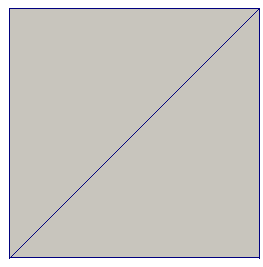
\includegraphics
    {beam_1_end}
  }
  \caption{Mesh for beam of size $0.01 \times 0.01\times 1$ with $1\times 1\times 10$ elements.}
\end{figure}

\begin{figure}[H]
  \centering
  \subfigure[Side View.]
  {
    
\includegraphics[width=1.0\textwidth]
    {beam_2}
  }
  \subfigure[End View.]
  {
    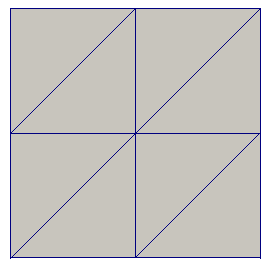
\includegraphics
    {beam_2_end}
  }
  \caption{Mesh for beam of size $0.01 \times 0.01\times 1$ with $2\times 2\times 20$ elements.
           Duplicated from Figure \ref{fig_mesh}.}
\end{figure}

\begin{figure}[H]
  \centering
  \subfigure[Side View.]
  {
    
\includegraphics[width=1.0\textwidth]
    {beam_4}
  }
  \subfigure[End View.]
  {
    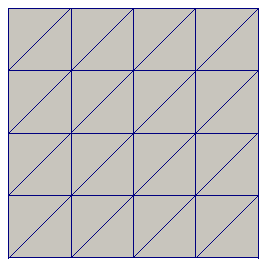
\includegraphics
    {beam_4_end}
  }
  \caption{Mesh for beam of size $0.01 \times 0.01\times 1$ with $4\times 4\times 40$ elements.}
\end{figure}

\begin{figure}[H]
  \centering
  \subfigure[Side View.]
  {
    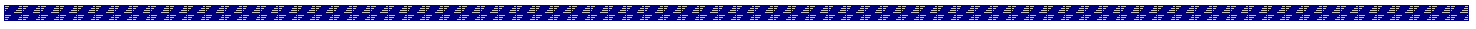
\includegraphics[width=1.0\textwidth]
    {beam_8}
  }
  \subfigure[End View.]
  {
    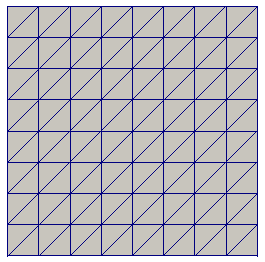
\includegraphics
    {beam_8_end}
  }
  \caption{Mesh for beam of size $0.01 \times 0.01\times 1$ with $8\times 8\times 80$ elements.}
\end{figure}

\end{document}
